%%%%%%%%%%%%%%%%%%%%%%%%%%%%%%%%%%%%%%%%%
% Developer CV
% LaTeX Template
% Version 1.0 (28/1/19)
%
% This template originates from:
% http://www.LaTeXTemplates.com
%
% Authors:
% Jan Vorisek (jan@vorisek.me)
% Based on a template by Jan Küster (info@jankuester.com)
% Modified for LaTeX Templates by Vel (vel@LaTeXTemplates.com)
%
% License:
% The MIT License (see included LICENSE file)
%
%%%%%%%%%%%%%%%%%%%%%%%%%%%%%%%%%%%%%%%%%

%----------------------------------------------------------------------------------------
%	PACKAGES AND OTHER DOCUMENT CONFIGURATIONS
%----------------------------------------------------------------------------------------

\documentclass[9pt]{developercv} % Default font size, values from 8-12pt are recommended
\usepackage{graphicx}
\usepackage[UKenglish]{babel}

%----------------------------------------------------------------------------------------

\begin{document}

%----------------------------------------------------------------------------------------
%	TITLE AND CONTACT INFORMATION
%----------------------------------------------------------------------------------------

\begin{minipage}[t]{0.4\textwidth} % 45% of the page width for name
	\vspace{-\baselineskip} % Required for vertically aligning minipages
	
	% If your name is very short, use just one of the lines below
	% If your name is very long, reduce the font size or make the minipage wider and reduce the others proportionately
	\colorbox{black}{{\HUGE\textcolor{white}{\textbf{\MakeUppercase{Mattia}}}}} % First name
	
	\colorbox{black}{{\HUGE\textcolor{white}{\textbf{\MakeUppercase{Piazza}}}}} % Last name
	
	\vspace{6pt}
	
	{\huge Researcher\\ Mechatronics Engineer} % Career or current job title
\end{minipage}
\begin{minipage}[t]{0.3\textwidth} % 27.5% of the page width for the first row of icons
	\vspace{-\baselineskip} % Required for vertically aligning minipages
	
	% The first parameter is the FontAwesome icon name, the second is the box size and the third is the text
	% Other icons can be found by referring to fontawesome.pdf (supplied with the template) and using the word after \fa in the command for the icon you want
	\icon{MapMarker}{10}{Maniago, PN, Italy}\\
	\icon{Globe}{10}{Italian}\\
	\icon{Phone}{10}{+39 333 15 14 344}\\
	%\icon{At}{10}{\href{mailto:piazzamattia1994@gmail.com}{piazzamattia1994@gmail.com}}\\
	\icon{At}{10}{\href{mailto:mattia.piazza@alumni.unitn.it}{mattia.piazza@unitn.it}}\\
	\icon{Linkedin}{10}{\href{https://www.linkedin.com/in/mattia-piazza-40167113b/}{mattia-piazza-40167113b}}\\
	%\icon{Skype}{10}{live:piazzamattia1994}\\
\end{minipage}
\hfill
\begin{minipage}[t]{0.2\textwidth} % 27.5% of the page width for the second row of icons
	\vspace{-\baselineskip} % Required for vertically aligning minipages
		\hfill
	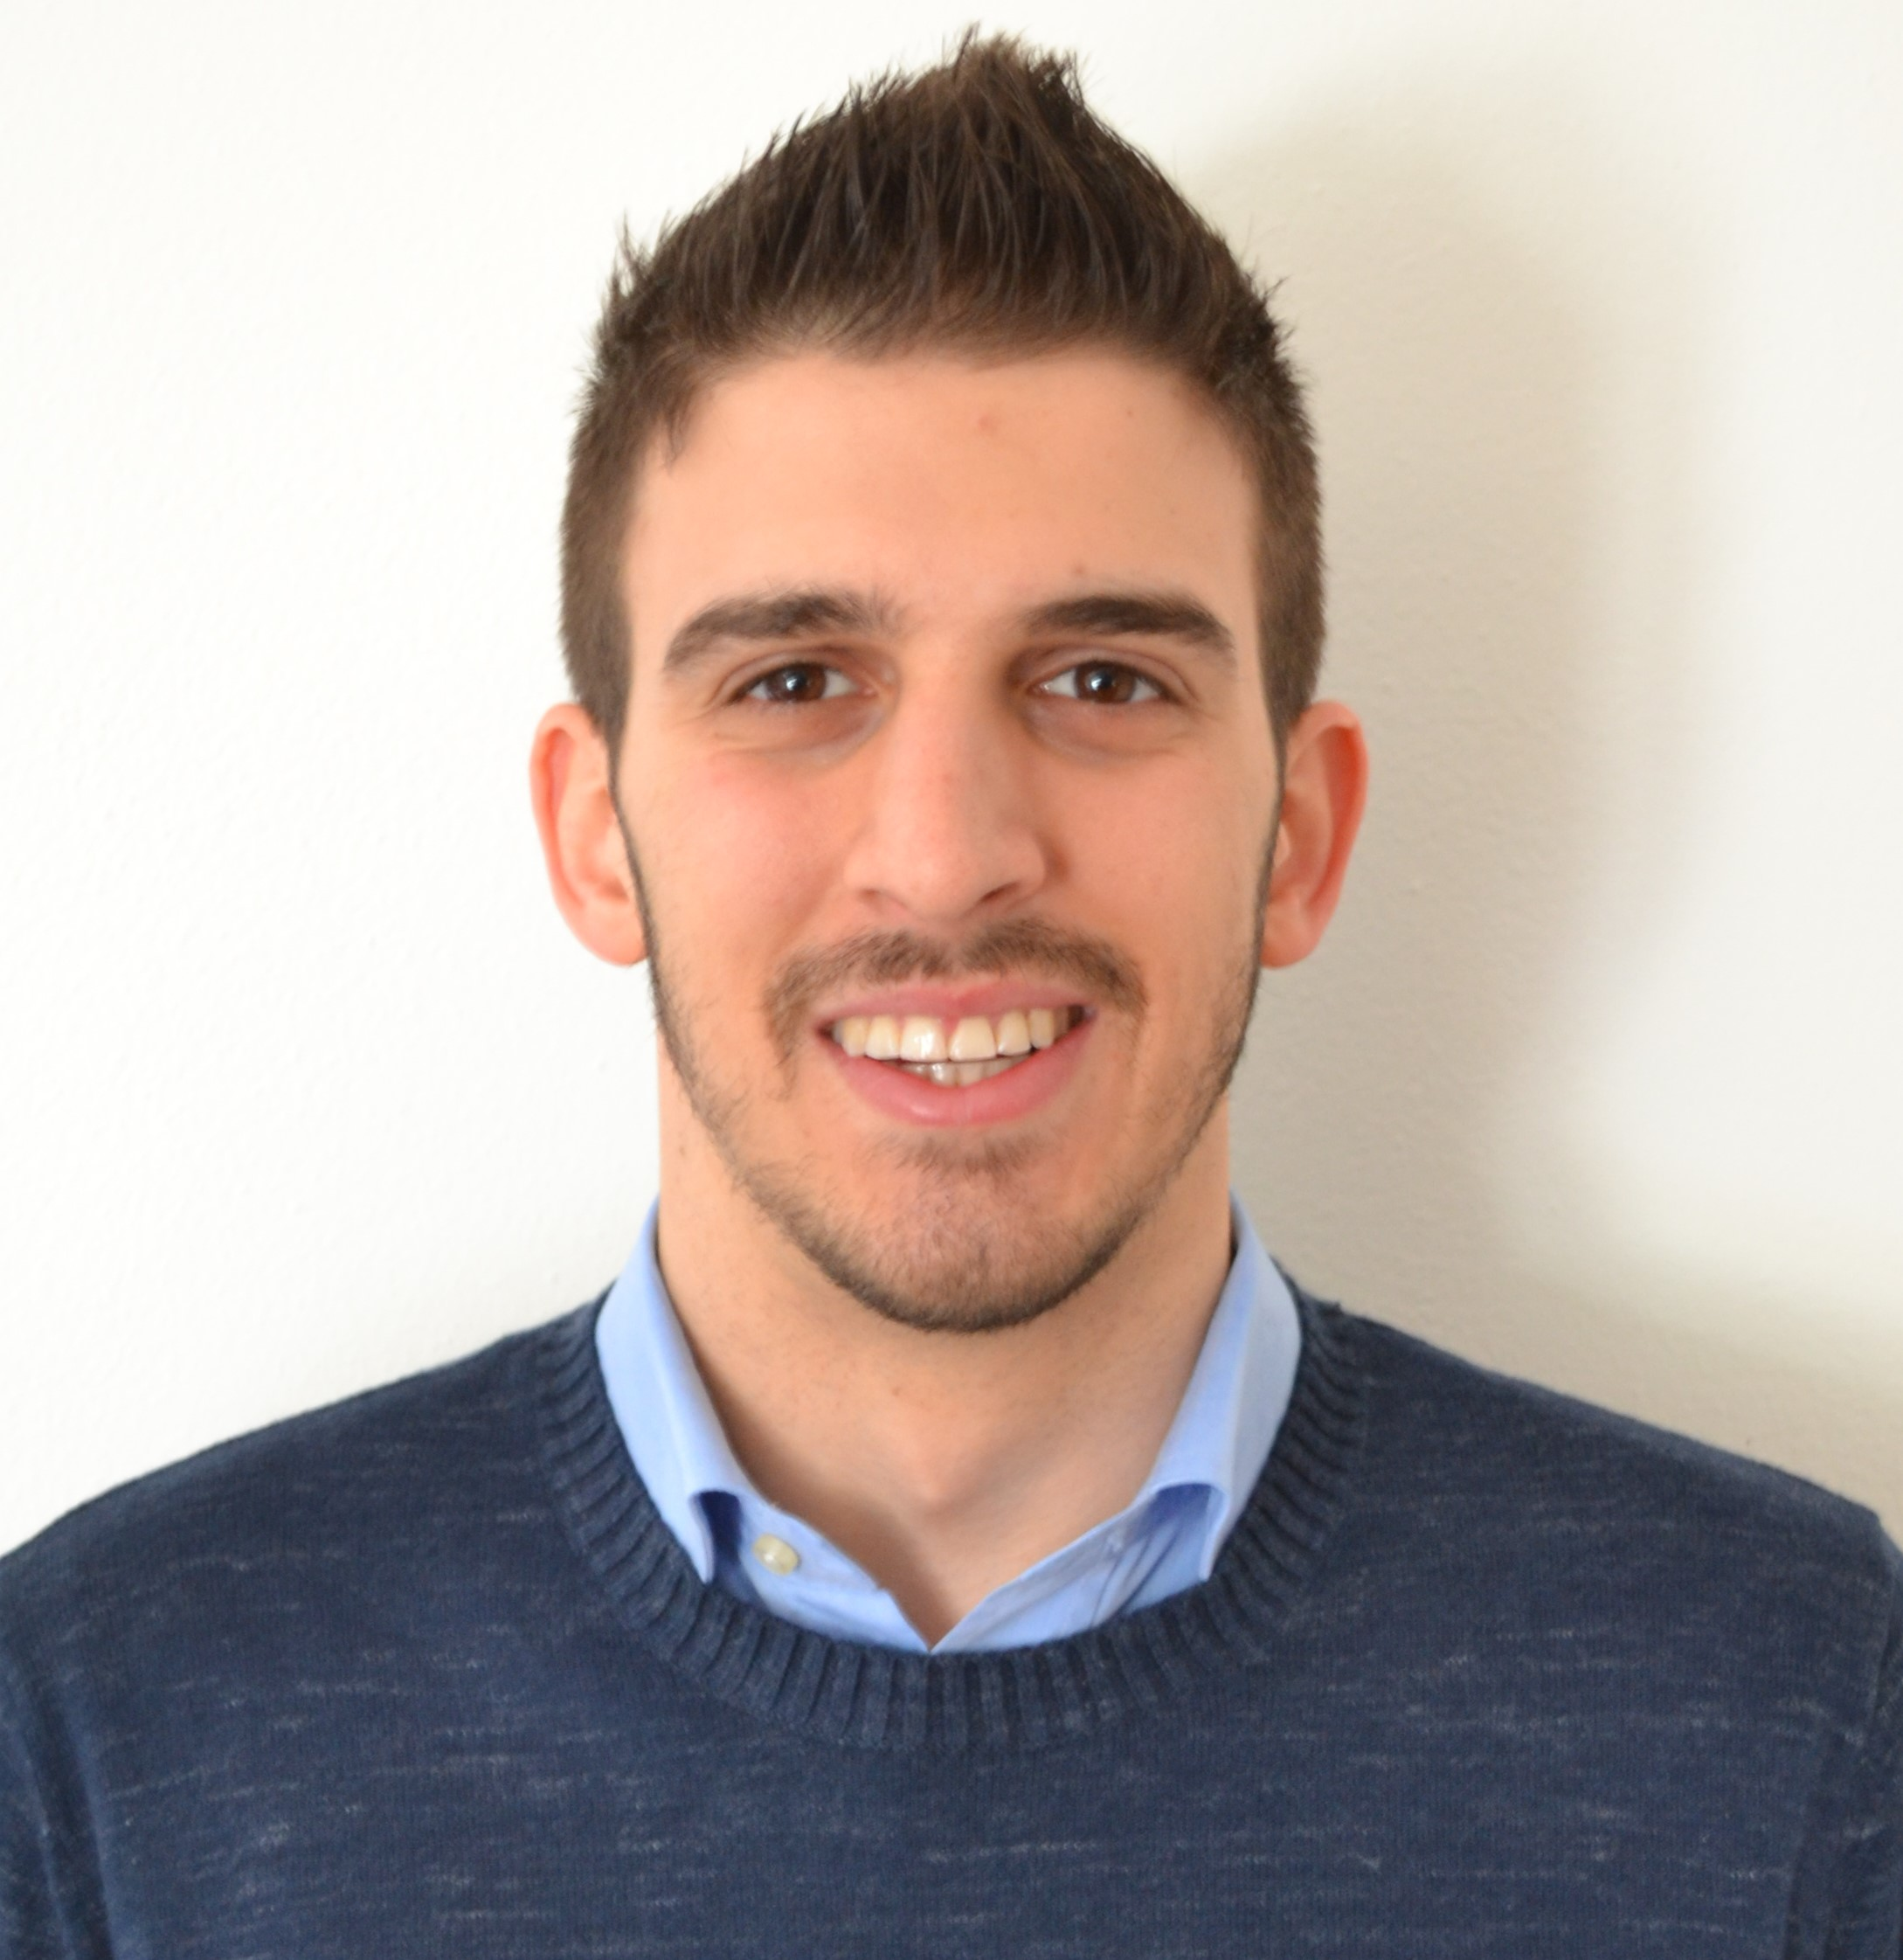
\includegraphics[width=1.0\linewidth]{Fototessera.jpg}
\end{minipage}
%
% \vspace{0.5cm}
%	INTRODUCTION, SKILLS AND TECHNOLOGIES
%
\cvsect{Who am I?}
%
\begin{minipage}[t]{0.5\textwidth} % 40% of the page width for the introduction text
	\vspace{-\baselineskip} % Required for vertically aligning minipages
%
I am a passionate mechatronics engineer who likes challenges and is always looking for personal growth opportunities. I am a determined man that is not afraid to leave his comfort zone to achieve goals and results. I am curious and always looking beyond appearances trying to optimise and put muy best effort at everything I do.
From the professional point of view, I am an expert in modelling and control of mechatronic systems with a particular focus at optimal control.
%
\end{minipage}
\hfill % Whitespace between
\begin{minipage}[t]{0.45\textwidth} % 50% of the page for the skills bar chart
	\vspace{-\baselineskip} % Required for vertically aligning minipages
	\begin{barchart}{5.5}
		\baritem{Maple}{100}
		\baritem{Matlab}{80}
		\baritem{C/C++}{60}
		\baritem{LaTeX}{70}
		\baritem{Python}{80}
		\baritem{Ruby}{40}
	\end{barchart}
\end{minipage}
%
% \begin{center}
% 	\bubbles{5/Inventor,3/AutoCAD, 4/ANSYS,3/Visual Studio}
% \end{center}
%
%	EXPERIENCE
%

\cvsect{Working Experiences}
%
\begin{entrylist}
	\entry
		{Jun.-Nov.2020}
		{Research scholarship}
		{University of Trento}
		{Research scholarship addressed to recent graduates (Decree n. 74/2020)\\ 
		Title: “Minimum Time Manoeuvres of complex vehicle models described with DAE".\\ 
		Supervisor: Prof. Francesco Biral.}
	\entry
		{Sept.--Dec. 2019 \&\\Sept.--Dec. 2018}
		{Tutorship specific areas for mechanics and mechatronics}
		{University of Trento}
		{Frontal lesson, lecture notes and exercises in English for freshmen students of the MSc in Mechatronics Engineering.\\
		Supervisors: Prof. Francesco Biral e Prof. Enrico Bertolazzi.}
	\entry
		{Apr.--Jun. 2019}
		{Video-lectures for the tutorship of mechanics and mechatronics}
		{University of Trento}
		{Development of video-lectures for the University with topic: linear algebra, scientific calculus, probability/statistics and mechanics.\\
		Supervisors: Prof. Daniele Fontanelli e Prof. Francesco Biral.}
	\entry
		{Jun.--Sept. 2017\\\footnotesize{Internship}}
		{Internship in Quality Control department}
		{SIAP s.p.a. gruppo CARRARO}
		{Precision measurements of mechanical components, development of sequential charts, specific control plans (SPC), CCP, measurements for capability analysis (Cp, Cpk, \textit{etc.}).
		}
	\entry
		{Jun.--Sept. 2013 \&\\Jun.--Sept. 2012}
		{Plumber apprentice}
		{DE NARDO ALESSANDRO IMPIANTI TERMOIDRAULICI}
		{Plumber apprentice during summer season.}
\end{entrylist}
%
%	EDUCATION
%
\cvsect{Education}
%
\begin{entrylist}
	\entry
		{2017 -- 2020}
		{Master of Science degree in Mechatronics Engineering}
		{University of Trento}
		{Curriculum mechanics e mechatronics. MSc offered entirely in English.\\
		Main courses: modeling and simulation of mechatronics systems, dynamic and control of vehicles and robots, mechanical design and machine elements, modeling with finite elements, industrial robotics.\hfill Grade:108/110}
		% computer vision, mechanical vibration,, automatic control
	\entry
		{2013 -- 2017}
		{Bachelor of Science degree in Mechanical Engineering}
		{University of Udine}
		{Main courses: Thermodynamics and heat transmission, applied mechanics, fluid-dynamics, Turbomachinery, Mechanics of solids and mechanical design, mechanical technology.} % \hfill Grade:94/110
	\entry
		{2008 -- 2013}
		{Scientific High school diploma}
		{Liceo Scientifico "Michelangelo Grigoletti"}
		{High school diploma with curriculum PNI (National Informatics Plan). } % \hfill Grade:67/100
\end{entrylist}
%
%	ADDITIONAL INFORMATION
%
\begin{minipage}[t]{0.3\textwidth}
	\vspace{-\baselineskip} % Required for vertically aligning minipages
	\cvsect{Lingue}
%
	\textbf{Italian} - Native\\
	\textbf{English}  - Fluent, C1 level (IELTS)
%
\end{minipage}
\hfill
\begin{minipage}[t]{0.3\textwidth}
	\vspace{-\baselineskip} % Required for vertically aligning minipages
	%
	\cvsect{Hobbies}
	%
	I am passionate about IoT, technology and smart gasgets. 
	I build and program small and automated projects with Arduino e Raspberry Pi.
%
\end{minipage}
\hfill
\begin{minipage}[t]{0.3\textwidth}
	\vspace{-\baselineskip} % Required for vertically aligning minipages
	%
	\cvsect{Sports}
%
	I am an amateur climber and a fairly good skier. %I also enjoy football and mountain trail running. 
%
\end{minipage}

\pagebreak 

%----------------------------------------------------------------------------------------

\cvsect{Privacy}

In compliance with the Italian Legislative Decree no. 196 dated 30/06/2003, I hereby authorize the recipient of this document to use and process my personal details for the purpose of recruiting and selecting staff and I confirm to be informed of my rights in accordance to art. 7 of the above mentioned decree.

\vspace{0.5cm}
Maniago, \today \\

\vspace{0.2cm}

\includegraphics[width=0.25\textwidth]{firma.jpg}


\end{document}
